\documentclass[11pt]{article}

\usepackage[a4paper,margin=0.8in]{geometry}

\usepackage{amsmath,amssymb,amsthm,mathtools}
\usepackage{bm}
\usepackage{hyperref, float}
\usepackage{xcolor}
\usepackage{microtype}
\usepackage[titletoc]{appendix}

\usepackage{titlesec}

\titleformat{\section}
{\large\bfseries}
{\thesection}
{0.5em}
{}

\titleformat{\subsection}
{\normalsize\bfseries}
{\thesubsection}
{0.5em}
{}

\titleformat{\subsubsection}
{\normalsize\itshape}
{\thesubsubsection}
{0.5em}
{}

\titlespacing*{\section}
{0pt}{1.2ex plus .2ex minus .2ex}{0.8ex}

\titlespacing*{\subsection}
{0pt}{1ex plus .2ex minus .2ex}{0.5ex}

\titlespacing*{\subsubsection}
{0pt}{0.8ex}{0.3ex}

% Slightly tighter spacing
\setlength{\parskip}{0.3em}
\setlength{\parindent}{0pt}

\setlength{\abovedisplayskip}{8pt}
\setlength{\belowdisplayskip}{8pt}

% Equations numbered by section
\numberwithin{equation}{section}

% Theorem numbering by section
\newtheorem{theorem}{Theorem}[section]
\newtheorem{proposition}[theorem]{Proposition}
\newtheorem{lemma}[theorem]{Lemma}
\newtheorem{corollary}[theorem]{Corollary}

\theoremstyle{definition}

\newtheorem{definition}[theorem]{Definition}
\newtheorem{example}[theorem]{Example}
\newtheorem{remark}[theorem]{Remark}

% Make theorem text upright instead of italic
\makeatletter
\def\th@plain{
  \normalfont
  \itshape
}
\makeatother

\newtheorem*{proposition*}{Proposition}

% Simple outline boxes
\usepackage{mdframed}

\surroundwithmdframed[
  linewidth=0.6pt,
  roundcorner=2pt,
  skipabove=10pt,
  skipbelow=10pt,
  innerleftmargin=8pt,
  innerrightmargin=8pt,
  innertopmargin=6pt,
  innerbottommargin=6pt
]{theorem}

\surroundwithmdframed[
  linewidth=0.6pt,
  roundcorner=2pt,
  skipabove=10pt,
  skipbelow=10pt,
  innerleftmargin=8pt,
  innerrightmargin=8pt,
  innertopmargin=6pt,
  innerbottommargin=6pt
]{proposition}

\surroundwithmdframed[
  linewidth=0.6pt,
  roundcorner=2pt,
  skipabove=10pt,
  skipbelow=10pt,
  innerleftmargin=8pt,
  innerrightmargin=8pt,
  innertopmargin=6pt,
  innerbottommargin=6pt
]{lemma}

\surroundwithmdframed[
  linewidth=0.6pt,
  roundcorner=2pt,
  skipabove=10pt,
  skipbelow=10pt,
  innerleftmargin=8pt,
  innerrightmargin=8pt,
  innertopmargin=6pt,
  innerbottommargin=6pt
]{corollary}

\surroundwithmdframed[
  linewidth=0.5pt,
  roundcorner=2pt,
  skipabove=10pt,
  skipbelow=10pt,
  innerleftmargin=8pt,
  innerrightmargin=8pt,
  innertopmargin=6pt,
  innerbottommargin=6pt
]{remark}

\surroundwithmdframed[
  linewidth=0.6pt,
  roundcorner=2pt,
  skipabove=10pt,
  skipbelow=10pt,
  innerleftmargin=8pt,
  innerrightmargin=8pt,
  innertopmargin=6pt,
  innerbottommargin=6pt
]{proposition*}

\newcommand{\X}{\mathcal{X}}

\title{Bounding weighted information gain -- first draft}
\author{Ajsa Jancar}
\date{May 2026}

\begin{document}

\maketitle

\textcolor{red}{Missing: \begin{itemize}
    \item References
\end{itemize}}

\newpage

\tableofcontents

\newpage 

\section{Introduction}

\paragraph{Classical information gain and active learning.}
In many active learning and Bayesian experimental design problems, the goal is not simply to collect observations, but to reduce uncertainty in a way that is useful for a downstream task. Classical information-gain objectives provide a useful measure of uncertainty reduction and have played a central role in Gaussian process active learning, Bayesian optimisation and experimental design. However, these objectives typically treat all parts of the domain uniformly. In many practical settings, uncertainty in some regions may be substantially more important than uncertainty elsewhere, suggesting that a more task-aware notion of information gain may be desirable.

\paragraph{Transductive Active Learning and task-aware exploration.}
Recent work on Transductive Active Learning (TAL) replaces the global objective with a target-dependent quantity
\begin{equation*}
\max_{X \subseteq S,\ |X|\leq T}
I(f_A;y_X),
\end{equation*}
which replaces the global objective with a target-dependent notion of information gain. Rather than measuring information acquired about the entire domain, TAL measures only the information gained about a specified target set. This allows exploration to focus on regions that are relevant to the downstream task and can lead to substantially sharper uncertainty bounds.

Despite this improvement, TAL still imposes a binary notion of relevance: points either belong to the target set or they do not. All locations within the target set are treated equally.

\paragraph{Motivating example.}

Consider an autonomous racing car learning the dynamics of a racetrack. Classical information-gain objectives encourage the vehicle to reduce uncertainty across the entire track, since all regions contribute equally to the objective. If the goal is simply to learn the track as accurately as possible everywhere, this behaviour is reasonable.

Suppose, however, that only a particular sequence of corners is safety-critical or performance-critical. In this setting, it is not obvious that the vehicle should continue allocating samples uniformly around the entire track. One may instead wish to prioritise uncertainty reduction in the important section while still accounting for information gained elsewhere.

TAL partially addresses this issue by allowing one to specify the critical section as a target set. However, all locations inside that section remain equally important. In practice, one might care most about a particular section of the corner, such as the point at which the vehicle begins braking, the turn-in point, or the point of maximum curvature, suggesting a more graded notion of task relevance.

\paragraph{Research question.}

This motivates the following question: can information gain be adapted to account for varying levels of importance across the domain while retaining useful theoretical structure?

Rather than specifying a binary target set, we seek a weighted notion of information gain in which different regions contribute according to a user-defined importance function. In this sense, the weighted setting may be viewed as a continuous analogue of the TAL framework.

\paragraph{A difficulty: loss of submodularity.}

A natural approach is to introduce weights directly into the marginal information gains, giving more importance to uncertainty reduction in some regions of the domain than in others. However, this modification fundamentally changes the structure of the objective.

For ordinary information gain, the objective can be written as a submodular set function, and the corresponding marginal gains satisfy a diminishing returns property. This structure underlies many of the theoretical guarantees in active learning and Bayesian experimental design, in particular allowing us to compare greedy selection objectives directly with maximum informatrion gain.

In the weighted setting, the contribution of an observation depends both on its weight and on its position in the observation sequence through the posterior variance. Consequently, the objective becomes order-dependent and can no longer be represented as a submodular set function. This prevents the direct application of the standard information-gain and transductive active learning framework, motivating the search for an alternative analytical approach.

\paragraph{Main contributions.}

The loss of submodularity means that weighted information gain cannot be analysed using the standard machinery underlying information gain and transductive active learning. Our main observation is that, despite this difficulty, piecewise constant weights admit a natural decomposition into regional information-gain terms.

\begin{proposition*}[Informal split bound]
Suppose the weight function is piecewise constant,
$$
w(x)
=
\sum_{i=1}^m
c_i \mathbf 1_{A_i}(x),
$$
for a partition
$
\mathcal X
=
\bigcup_{i=1}^m A_i.
$
Then the weighted information gain can be bounded by a sum of ordinary information-gain terms on the individual regions, each evaluated with an effective noise level proportional to $\sigma^2/c_i^2$.
\end{proposition*}

This result reduces the analysis of weighted information gain to the analysis of standard information gain on individual regions. Consequently, existing information-gain bounds for Gaussian process kernels can be applied separately on each region, allowing the effects of geometry, volume and intrinsic dimension to be captured explicitly. In particular, the resulting bounds reveal situations in which weighted exploration can be substantially more efficient than global exploration, especially when highly weighted regions occupy only a small subset of the domain or lie on lower-dimensional structures.

\begin{proposition*}[Informal consequence for Squared Exponential kernels]
For Squared Exponential kernels, applying the split bound reveals that restricting attention to smaller regions primarily affects lower-order geometric constants. In particular, regional volume enters only logarithmically into the resulting information gain bounds. Consequently, the largest improvements arise when highly weighted regions have lower effective dimension than the ambient domain.
\end{proposition*}

\begin{proposition*}[Informal consequence for Mat\'ern kernels]
For Mat\'ern kernels, applying the split bound reveals a substantially stronger dependence on regional geometry. Both the volume of a region and its effective dimension influence the leading-order information gain rate. Consequently, concentrating weight on small or lower-dimensional regions can improve not only constants but also the polynomial scaling of the information gain bound.
\end{proposition*}

The remainder of the paper formalises this decomposition, establishes weighted information-gain bounds for piecewise constant weight functions and investigates how regional geometry and intrinsic dimension affect the resulting rates for linear, Squared exponential and Matérn kernels.



\section{Weighted information gain}

In the standard Gaussian process setting, the maximum information gain after $T$ observations is
\begin{equation*}
\Gamma_T
= \frac{1}{2}
\max_{x_1,\dots,x_T}
\sum_{t=1}^T
\log\!\left(
1+\frac{\sigma_{t-1}^2(x_t)}{\sigma^2}
\right),
\end{equation*}
where $\sigma_{t-1}^2(x_t)$ denotes the posterior variance before observing $x_t$.

Motivated by the preceding discussion, we introduce the weighted sequential objective
\begin{equation*}
\Gamma_T^w
= \frac{1}{2}
\sum_{t=1}^T
w(x_t)^2
\log\!\left(
1+\frac{\sigma_{t-1}^2(x_t)}{\sigma^2}
\right).
\end{equation*}

The weights act externally on the marginal gains while leaving the Gaussian process posterior unchanged. The motivation is that if $w$ is concentrated on a sufficiently small subset of the domain, then $\Gamma_T^w$ may admit sharper bounds than the ordinary information gain.
For example, if
\begin{equation*}
w(x)=c\,\mathbf{1}_A(x),
\end{equation*}
then
\begin{equation*}
\Gamma_T^w
= \frac{c^2}{2}
\sum_{t:\,x_t\in A}
\log\!\left(
1+\frac{\sigma_{t-1}^2(x_t)}{\sigma^2}
\right),
\end{equation*}
which resembles a transductive information gain restricted to $A$.

\subsection{Loss of submodularity for weighted objective}

For ordinary information gain, the set function
\begin{equation*}
F(S)=I(f_S;y_S)
\end{equation*}
has marginal gains
\begin{equation*}
F(S\cup\{x\})-F(S)
=
\frac12
\log\!\left(
1+\frac{\sigma_S^2(x)}{\sigma^2}
\right),
\end{equation*}
which satisfy diminishing returns. This submodularity is what allows standard greedy approximation arguments.

The weighted objective does not inherit this structure. Writing formally
\begin{equation*}
F_w(x_1,\dots,x_T)
= \frac{1}{2}
\sum_{t=1}^T
w(x_t)^2
\log\!\left(
1+\frac{\sigma_{t-1}^2(x_t)}{\sigma^2}
\right),
\end{equation*}
the contribution of a point depends both on its weight and on its position in the sequence through the posterior variance. As a result, the objective is order-dependent and thus cannot be expressed as a submodular set function.This prevents the direct application of the standard TAL framework.

\section{A first attempt: kernel reweighting}

An initial idea to recover submodularity was to incorporate the weights directly into the kernel by defining
\begin{equation*}
k_w(x,x')
=
w(x)\,k(x,x')\,w(x').
\end{equation*}
The corresponding information gain then becomes
\begin{equation*}
\Gamma_T(k_w)
=
\max_{x_1,\dots,x_T} \frac{1}{2}
\log
\det
\left(
I+\sigma^{-2}K_T^{(w)}
\right),
\end{equation*}
where
\begin{equation*}
K_T^{(w)}(i,j)
=
w(x_i)k(x_i,x_j)w(x_j).
\end{equation*}

This restores submodularity, since the objective is again ordinary Gaussian process information gain. However, the Gaussian process prior itself has changed. The posterior variance now satisfies
\begin{equation*}
\sigma_{n,w}^2(x)
=
k_w(x,x)
-
k_w(x,X_n)
\left(
K_n^{(w)}+\sigma^2 I
\right)^{-1}
k_w(X_n,x),
\end{equation*}
which is not equal to
\begin{equation*}
w(x)^2\sigma_n^2(x).
\end{equation*}
Thus the weighting modifies the geometry of the Gaussian process itself rather than only the acquisition objective. This leads to the assumption that higher-weighted regions have inherently larger variance (amplitude of $f$), changing the posterior itself and altering predicitions. Therefore, the resulting optimisation problem is fundamentally different from the original weighted formulation and we are no longer solving the original problem. 

\section{Second attempt: piecewise weighted objectives} 

A second approach was to define a weighted objective at the level of disjoint regions. 

\subsection{A weighted sum of regional objectives}

We proceed as follows: let $\X$ be a domain and $A_1, \ldots A_m$ a partition of $\X$ so that
\begin{equation*}
\X=\bigcup_{i=1}^m A_i,
\qquad
A_i \cap A_j = \emptyset \quad \text{for} \quad i \neq j.
\end{equation*}
We consider a piecewise constant weighting function:
\begin{equation*}
w(x)=\sum_{i=1}^m c_i\mathbf{1}_{A_i}(x).
\end{equation*}
One may then define the weighted objective on a queried set $S \subseteq \X$ by
\begin{equation*}
F_w(S)
=
\sum_{i=1}^m
c_i\,I(f_{A_i};y_S) = \sum_{i=1}^m
c_i F_{A_i}(S).
\end{equation*}

\subsection{Submodularity of the regional objective}

We claim that $F_w(\cdot)$ defined this way is a submodular setfunction. Indeed, if we consider subsets $A \subseteq B \subseteq \X$, $x \notin B$ and define the marginal gain $\Delta_w(x \mid \cdot) := F_w(\cdot \cup \{x\}) - F_w(\cdot)$, then
\begin{align*}
    \Delta_w(x \mid \cdot) &= \sum_{i=1}^m c_i \left( I(f_{A_i}; y_{\; \cdot \; \cup \{x\}}) - I(f_{A_i}; y_{\; \cdot \;}) \right) \\
    &= \sum_{i=1}^m c_i \Delta_i(x \mid \cdot) \\
    &= \sum_{i=1}^m c_i \left(F_{A_i}(\cdot \cup \{x\}) - F_{A_i}(\cdot)\right).
\end{align*}
Now since each $F_{A_i}$ is submodular, for every $I$, when $A\subseteq B$, $\Delta_i(x \mid A) \geq \Delta_i(x \mid B)$ so that 
\begin{equation*}
    \Delta_w(x \mid A) = \sum_i c_i \Delta_i(x \mid A) \geq \sum_i c_i \Delta_i(x \mid B) = \Delta_w(x \mid B).
\end{equation*}
Thus, the entire objective remains submodular and greedy selection inherits the usual approximation guarantee
\begin{equation*}
F_w(S_{\mathrm{greedy}})
\geq
(1-e^{-1})
\max_{|S|\leq T}
F_w(S).
\end{equation*}
We have shown the following proposition:
\begin{proposition} \label{prop: submodularobj}
    Let $w(x)=\sum_{i=1}^m c_i\mathbf{1}_{A_i}(x)$ with $c_i \geq 0$ and define 
    $$F_w(S)=
    \sum_{i=1}^m
    c_i\,I(f_{A_i};y_S).$$ 
    If each $S \to I(f_{A_i}; y_S)$ is submodular, then $F_w$ is submodular.
\end{proposition}

\subsection{Why this doesn't work for our weighted objective}
The objective defined above differs from the original sequential weighted information gain: instead of weighting the marginal gains directly, it weights independent transductive objectives over different regions. This is illustrated below.

Recall our objective
\begin{equation*}
F(S)
= \frac{1}{2}
\sum_{n=1}^{|S|}
\log\!\left(
1+w(x_n)^2\,\sigma_{n-1}^2(x_n).
\right)
\end{equation*}
If we introduce piecewise weights as above, this becomes
\begin{equation*}
F(S)
= \frac{1}{2}
\sum_n
\log\!\left(
1+c_{\mathrm{region}(z_n)}^2
\cdot
\sigma_{n-1}^2(x_n)
\right),
\end{equation*}
where $\sigma_{n-1}^2(x_n)$
depends on all previously selected points across all regions.
Even if we force a decomposition by region,
\begin{equation*}
F(S)
= \frac{1}{2}
\sum_i
\sum_{x_n \in A_i}
\log\!\left(
1+c_i^2
\sigma_{n-1}^2(x_n)
\right),
\end{equation*}
this is still not a function only of the set, because
$\sigma_{n-1}^2(z_n)$
depends on which points were chosen earlier and in which order, including points from other regions.

The proposition requires weights to act on independent components of the objective; in our objective, the weights instead act on sequential updates coupled through the GP posterior. This motivates the idea in Section \ref{sec: indepregions}.

\subsection{A possible solution: regional transductive objective} \label{sec: transobjective}

A natural way to recover submodularity is to move the weighting from the sequential marginal gains to the transductive objectives themselves. Suppose the domain is partitioned into disjoint regions
\begin{equation*}
A_1,\dots,A_m \subseteq \mathcal{X}.
\end{equation*}
Rather than weighting posterior variance updates directly, we instead define a weighted sum of regional information gains. The resulting objective takes the form
\begin{equation} \label{eq: regionaltransductiveobj}
F_w(S)
=
\sum_{i=1}^m
c_i\, I(f_{A_i};y_S),
\end{equation}
where
\begin{equation*}
I(f_{A_i};y_S)
=
H(f_{A_i})
-
H(f_{A_i}\mid y_S)
=
\frac12
\log\!\left(
\frac{\det K_{A_i,A_i}}
{\det K_{A_i,A_i\mid S}}
\right)
\end{equation*}
and
\begin{equation*}
K_{A_i,A_i\mid S}
=
K_{A_i,A_i}
-
K_{A_i,S}
\left(
K_{S,S}+\sigma^2 I
\right)^{-1}
K_{S,A_i}.
\end{equation*}
This formulation replaces the sequential variance-weighted updates with a weighted sum of regional transductive information gains, where each term measures the information gained about a fixed target region $A_i$ and the coefficients $c_i$ determine their relative importance. Since mutual information is submodular as a function of the observation set $S$, by Proposition \ref{prop: submodularobj}, the resulting objective inherits the standard greedy approximation guarantees. 

Conceptually, the key distinction between this objective and the original weighted sequential information gain is that in \eqref{eq: regionaltransductiveobj}, the weights act on the target of the information gain rather than on the locations from which observations are collected. Since mutual information is symmetric, the weighted objective remains a nonnegative combination of mutual information quantities, and the submodular structure is preserved. By contrast, in the original sequential weighted objective, the weights act directly on the individual variance reductions according to where the observations are taken from, introducing order dependence and breaking the symmetry.

Although this objective is not equivalent to the original weighted sequential information gain, the regional structure introduced here will later motivate the decomposition bound derived in Section \ref{sec: splitbound}.
\subsection{Extending to continuous weighting}

The piecewise-constant formulation in \eqref{eq: regionaltransductiveobj} suggests a possible route toward continuous weighting functions. Informally, one may approximate a continuous weight function by increasingly fine partitions of the domain and consider the corresponding weighted regional transductive objectives. In the limit, one might hope to recover a continuum version of the weighted information gain.

Heuristically, if the regions shrink to points, the regional mutual information terms should converge to local information quantities, leading formally to an objective of the form
\begin{equation*}
\int
w(x)\,
I(f(x);y_S)\,
d\mu(x).
\end{equation*}

For Gaussian processes,
\begin{equation*}
I(f(x);y_S)
=
\frac12
\log\!\left(
1+\frac{\sigma_S^2(x)}{\sigma^2}
\right),
\end{equation*}
so this becomes
\begin{equation*}
\frac12
\int
w(x)
\log\!\left(
1+\frac{\sigma_S^2(x)}{\sigma^2}
\right)
d\mu(x),
\end{equation*}
which may be interpreted as a weighted integrated information density over the domain.

Moreover, in the small-variance regime,
\begin{equation*}
\log(1+t)\approx t,
\end{equation*}
giving the approximation
\begin{equation*}
\frac12
\int
w(x)
\log\!\left(
1+\frac{\sigma_S^2(x)}{\sigma^2}
\right)
d\mu(x)
\approx
\frac1{2\sigma^2}
\int
w(x)\sigma_S^2(x)\,d\mu(x),
\end{equation*}
which resembles a weighted integrated posterior variance criterion commonly appearing in Bayesian experimental design and active learning.

However, there is an important structural distinction. The finite-dimensional piecewise objective
\begin{equation*}
F_w(S)
=
\sum_i
c_i I(f_{A_i};y_S)
\end{equation*}
inherits submodularity from mutual information, and therefore retains the usual greedy approximation guarantees. By contrast, integrated variance objectives are not naturally submodular and do not generally admit the same diminishing returns structure.
Thus, while the continuum limit formally resembles an integrated variance functional, it is not clear whether the submodular structure survives after passing to the limit.

A more detailed heuristic approximation argument is deferred to Appendix~\ref{appendix:continuum}.

\subsection{Special case: independent regions} \label{sec: indepregions}

The regional transductive formulation \eqref{eq: regionaltransductiveobj} becomes particularly natural in the case where different regions are independent under the kernel. In this setting, observations from one region do not influence uncertainty in another, so the regional objectives decouple completely.

If distinct regions are independent under the kernel, namely
\begin{equation*}
k(x,x')=0
\qquad
\text{for } x\in A_i,\ x'\in A_j,\ i\neq j,
\end{equation*}
then the information gain decomposes additively:
\begin{equation*}
I(f_A;y_X)
=
\sum_{i=1}^m
I(f_{A_i};y_{X\cap A_i}).
\end{equation*}
In this case,
\begin{equation*}
F_w(S)
=
\sum_{i=1}^m
c_i
I(f_{A_i};y_{S\cap A_i}),
\end{equation*}
and the optimisation problem separates exactly across regions.

Although unrealistic in general, this illustrates the mechanism underlying the regional decomposition. In the independent case, the weighted objective separates exactly across regions. In the general correlated setting, this exact decomposition fails due to coupling through the GP, but the same intuition still leads to a useful upper bound on the original weighted information gain. We see this in the next section.

\section{Split bound} \label{sec:splitbound}

We now derive an upper bound on the weighted information gain
$\Gamma_T^w$ by exploiting spatial structure in the weighting function.
The regional transductive formulation discussed in
Appendix~\ref{app:transobjective} provides intuition for why decomposing
the domain into regions can be useful, while the independent-regions case
in Appendix~\ref{app:indepregions} shows that such decompositions become
exact when the Gaussian process does not couple different regions.

In the general setting, regions are correlated through the kernel and an
exact decomposition is no longer possible. Nevertheless, a similar idea
can be used to obtain an upper bound. The key observation is that posterior
variance can only decrease when conditioning on additional observations.
Consequently, the contribution from a region can be bounded by considering
only the subsequence of observations lying inside that region.

This leads to a decomposition of $\Gamma_T^w$ into regional information
gain terms with rescaled effective noise variances. Intuitively, larger
weights correspond to smaller effective noise levels, and therefore to
larger regional information gains.

\subsection{Statement of the split bound}

\begin{proposition}[Split bound for piecewise constant weights] \label{prop: splitbound}
Let $\mathcal{X}=\bigcup_{i=1}^m A_i$ be a disjoint partition, and let
\begin{equation*}
w(x)
=
\sum_{i=1}^m
c_i\mathbf{1}_{A_i}(x).
\end{equation*}
Then the weighted information gain satisfies
\begin{equation*}
\Gamma_T^w
\leq
\max_{T_1+\cdots+T_m=T}
\sum_{i=1}^m
\Gamma_{A_i}^{\mathrm{unweighted}}
\left(
T_i;\frac{\sigma^2}{c_i^2}
\right),
\end{equation*}
where $\Gamma_{A_i}^{\mathrm{unweighted}}(T_i;\sigma^2/c_i^2)$ denotes the ordinary information gain restricted to $A_i$ with effective noise variance $\sigma^2/c_i^2$.
\end{proposition}

\begin{remark}[Effective noise interpretation]
The split bound may be interpreted as decomposing the weighted information gain into regional information gain problems with rescaled noise levels. Larger weights correspond to smaller effective noise variances and therefore larger regional information gains.
\end{remark}

\subsection{Proof in the two-region case}

\begin{proof}[Proof of Proposition \ref{prop: splitbound}, two-region case]
We first prove the claim in the simple case where the ambient space is partitioned into two regions. Let
\begin{equation*}
w(z)
=
a\,\mathbf{1}_A(z)
+
b\,\mathbf{1}_B(z),
\end{equation*}
where
\begin{equation*}
A\cap B=\varnothing,
\qquad
A\cup B=\mathcal{X}.
\end{equation*}
Define
\begin{equation*}
\Gamma_A(N;a)
:= \frac{1}{2}
\max_{x_1,\dots,x_N\in A}
\sum_{j=1}^N
\log\!\left(
1+
\frac{a^2}{\sigma^2}
\tilde{\sigma}_{j-1,A}^2(x_j)
\right),
\end{equation*}
where $\tilde{\sigma}_{j-1,A}^2(x)$ denotes the posterior variance obtained by conditioning only on the previously selected points lying in $A$ (rather than on the full observation sequence)
and similarly
\begin{equation*}
\Gamma_B(N;b)
:= \frac{1}{2}
\max_{x_1,\dots,x_N\in B}
\sum_{j=1}^N
\log\!\left(
1+
\frac{b^2}{\sigma^2}
\tilde{\sigma}_{j-1,B}^2(x_j)
\right).
\end{equation*}
Take a sequence $z_1,\dots,z_N,$
and suppose there are $m$ points in $A$ and $N-m$ points in $B$.
Write the $A$-subsequence as $z_{t_1},\dots,z_{t_m}$
in order of appearance in the full sequence. Then its contribution is
\begin{equation*}
\sum_{j=1}^m
\log\!\left(
1+
\frac{a^2}{\sigma^2}
\tilde{\sigma}_{t_j-1,\mathcal{X}}^2(z_{t_j})
\right).
\end{equation*}
Now since $\tilde{\sigma}_{t_j-1,\mathcal{X}}^2(z_{t_j})
\leq
\tilde{\sigma}_{j-1,A}^2(z_{t_j}),$
(as conditioning on additional points can only reduce posterior variance),
\begin{equation*} \frac{1}{2}
\sum_{j=1}^m
\log\!\left(
1+
\frac{a^2}{\sigma^2}
\tilde{\sigma}_{t_j-1,\mathcal{X}}^2(z_{t_j})
\right)
\leq \frac{1}{2}
\sum_{j=1}^m
\log\!\left(
1+
\frac{a^2}{\sigma^2}
\tilde{\sigma}_{j-1,A}^2(z_{t_j})
\right)
\leq
\Gamma_A(m;a).
\end{equation*}
The same argument applies to the $B$-subsequence, giving
\begin{equation*}
\Gamma_N(w,k)
\leq
\Gamma_A(m;a)
+
\Gamma_B(N-m;b).
\end{equation*}
Taking the maximum over all allocations $m$ yields
\begin{equation*}
\Gamma_N(w,k)
\leq
\max_{m=0,\dots,N}
\left\{
\Gamma_A(m;a)
+
\Gamma_B(N-m;b)
\right\}.
\end{equation*}
Now observe that
\begin{equation*}
\Gamma_A(m;a)
=
\Gamma_A^{\mathrm{unweighted}}
\!\left(
m;
\left(\frac{\sigma}{a}\right)^2
\right),
\end{equation*}
corresponding to ordinary information gain on $A$ with effective noise variance
$\sigma_A^2
=
\frac{\sigma^2}{a^2}.$
Similarly,
\begin{equation*}
\Gamma_B(N-m;b)
=
\Gamma_B^{\mathrm{unweighted}}
\!\left(
N-m;
\left(\frac{\sigma}{b}\right)^2
\right).
\end{equation*}
Hence
\begin{equation*}
\Gamma_N(w,k)
\leq
\max_{m=0,\dots,N}
\left\{
\Gamma_A^{\mathrm{unweighted}}
\!\left(
m;
\left(\frac{\sigma}{a}\right)^2
\right)
+
\Gamma_B^{\mathrm{unweighted}}
\!\left(
N-m;
\left(\frac{\sigma}{b}\right)^2
\right)
\right\}.
\end{equation*}
Equivalently, in log-determinant form,
\begin{equation*}
\Gamma_A^{\mathrm{unweighted}}
\!\left(
m;
\left(\frac{\sigma}{a}\right)^2
\right)
= \frac{1}{2}
\max_{S\subseteq A,\ |S|=m}
\log\det
\left(
I+\sigma_A^{-2}K_{S,S}
\right),
\end{equation*}
so that
\begin{equation*}
\Gamma_N(w,k)
\leq \frac{1}{2}
\max_{m=0,\dots,N}
\Bigg\{
\max_{S\subseteq A,\ |S|=m}
\log\det
\left(
I+\left(\frac{\sigma}{a}\right)^{-2}
K_{S,S}
\right)
\end{equation*}

\begin{equation*}
\qquad\qquad
+
\max_{Y\subseteq B,\ |Y|=N-m}
\log\det
\left(
I+\left(\frac{\sigma}{b}\right)^{-2}
K_{Y,Y}
\right)
\Bigg\}.
\end{equation*}
\end{proof}

\subsection{Extension to finitely many regions}
\begin{proof}[Proof of Proposition \ref{prop: splitbound}, general case]
The same argument extends to finitely many disjoint regions. Let
\begin{equation*}
\mathcal{X}
=
\bigcup_{i=1}^m A_i,
\qquad
A_i\cap A_j=\varnothing
\quad
(i\neq j),
\end{equation*}
and define
\begin{equation*}
w(x)
=
\sum_{i=1}^m
c_i\mathbf{1}_{A_i}(x).
\end{equation*}
If $T_i$ denotes the number of sampled points in region $A_i$, with $T_1+\cdots+T_m=T,$
then applying the subsequence argument region-by-region gives
\begin{equation*}
\Gamma_T^w
\leq
\max_{T_1+\cdots+T_m=T}
\sum_{i=1}^m
\Gamma_{A_i}^{\mathrm{unweighted}}
\left(
T_i;\frac{\sigma^2}{c_i^2}
\right).
\end{equation*}
Equivalently, each region behaves like an independent information gain problem with effective noise level
$
\sigma_i^2
=
\frac{\sigma^2}{c_i^2}.$
\end{proof}

Unlike the exact decomposition in the independent-region setting, this bound remains valid even when correlations between regions are present. In the independent-region setting of Appendix \ref{app:indepregions}, the inequalities above become equalities, since observations outside a region no longer affect the posterior variances within it.


\subsection{Comparison with the crude bound}

The crude bound corresponds to replacing the weight function by its maximum value everywhere. If $a\geq b$, this gives
\begin{equation*}
B_{\mathrm{crude}}
:=
\Gamma_N^{\mathrm{unweighted}}
\left(k;\frac{\sigma^2}{a^2}\right)
= \frac{1}{2}
\max_{|S|=N}
\log\det
\left(
I+\frac{a^2}{\sigma^2}K_{S,S}
\right).
\end{equation*}
By contrast, the split bound from Proposition \ref{prop: splitbound} keeps track of how many samples fall in each region:
\begin{equation*}
B_{\mathrm{split}}
:=
\max_{m=0,\dots,N}
\left\{
\Gamma_A^{\mathrm{unweighted}}
\left(m;\frac{\sigma^2}{a^2}\right)
+
\Gamma_B^{\mathrm{unweighted}}
\left(N-m;\frac{\sigma^2}{b^2}\right)
\right\}.
\end{equation*}
The crude bound treats the whole domain as if it had the largest weight $a$, while the split bound only applies this effective noise level inside $A$ and uses the smaller effective weight in $B$.

With this decomposition, we hope to exploit geometric differences between regions. In particular, if highly weighted regions occupy smaller subsets of the domain, the associated information gain terms may decay more rapidly.

\subsection{Alternative weighting approaches}

The split bound exploits spatial structure in $w$ while leaving the
Gaussian process model unchanged. We contrast this with two alternative
ways of incorporating task relevance, discussed in detail in
Appendices~\ref{app:weighted_kernel} and
\ref{app:regional_objective}.

First, one could absorb the weights directly into the kernel by defining
$$
k_w(x,x')
=
w(x)w(x')k(x,x').
$$
For this modified kernel, the standard information gain machinery applies
directly. However, as discussed in Appendix~\ref{app:weighted_kernel}, this
changes the geometry of the Gaussian process prior rather than only changing
the acquisition objective. In particular, the posterior variances under the
weighted kernel do not generally satisfy
$$
\sigma_{t,w}^2(x)
=
w(x)^2\sigma_t^2(x).
$$
Therefore, kernel weighting corresponds to solving a different regression
problem: the notion of similarity between points is changed by the relevance
weights, rather than only changing which uncertainties are important.

Second, one can define a regional objective by applying weights to
transductive information gains over different target regions. Thus, the weighting is applied to the target region where uncertainty should be
reduced, rather than to the locations chosen for sampling. Given a
partition $\{A_i\}_{i=1}^m$ of set $S$], this gives
\[
F_w(S)
=
\sum_{i=1}^m c_i I(f_{A_i};y_S).
\]
Each term is submodular  and since nonnegative
sums of submodular functions remain submodular, the objective preserves
the usual greedy guarantees (see Appendix~\ref{app:regional_objective}).
However, this represents a different notion of task relevance: the
weights act on the prediction targets rather than directly on the
sequential variance reductions. 

The weighted acquisition objective studied here instead weights the marginal
value of reducing uncertainty at each sampled location. This allows a
graded notion of relevance across $\mathcal X$ while leaving the Gaussian
process posterior unchanged.


\section{Computational illustration}

To illustrate the behaviour of the split bound, we consider a simple
Gaussian process design problem on a finite candidate set.

We sample $M=3000$ candidate locations uniformly from $[0,1]^2$
and select a budget of $N=100$ observations.
The underlying Gaussian process uses a squared exponential kernel with
lengthscale $\ell=0.12$, unit signal variance and observation noise
variance $\sigma^2=0.02$.

In both experiments below we compare a smooth Gaussian weight function
with a piecewise constant two-region overestimate. The latter is chosen
so that
\begin{equation*}
w_{\mathrm{clip}}(x)\geq w_{\mathrm{gauss}}(x)
\end{equation*}
for every candidate location, allowing the split bound developed in the
previous sections to be applied.

Since exact computation of maximum information gain is combinatorial in
the number of candidate points, all information-gain quantities reported
here are greedy approximations. The purpose of the experiment is not to
estimate the exact values of the bounds, but rather to investigate how
the split bound behaves relative to the corresponding crude bound.
\subsection{Localised high-weight region}

We first consider a Gaussian weight centred at a single point,
\begin{equation*}
w_{\mathrm{gauss}}(x)
=
a\exp\!\left(
-\frac{\|x-c\|^2}{2s^2}
\right),
\end{equation*}
with
\begin{equation*}
a=2,
\qquad
c=(0.78,0.72),
\qquad
s=0.10.
\end{equation*}

As before, we construct a two-region overestimate
\begin{equation*}
w_{\mathrm{clip}}(x)
=
\begin{cases}
a,& \|x-c\|\le r,\\
b,& \text{otherwise},
\end{cases}
\end{equation*}
with $b=0.5$ and
\begin{equation*}
r=s\sqrt{2\log(a/b)}.
\end{equation*}

This partitions the domain into a high-weight region $A$ and a background region $B$, containing $256$ and $2744$ candidate points respectively.

\begin{figure}[H]
\centering
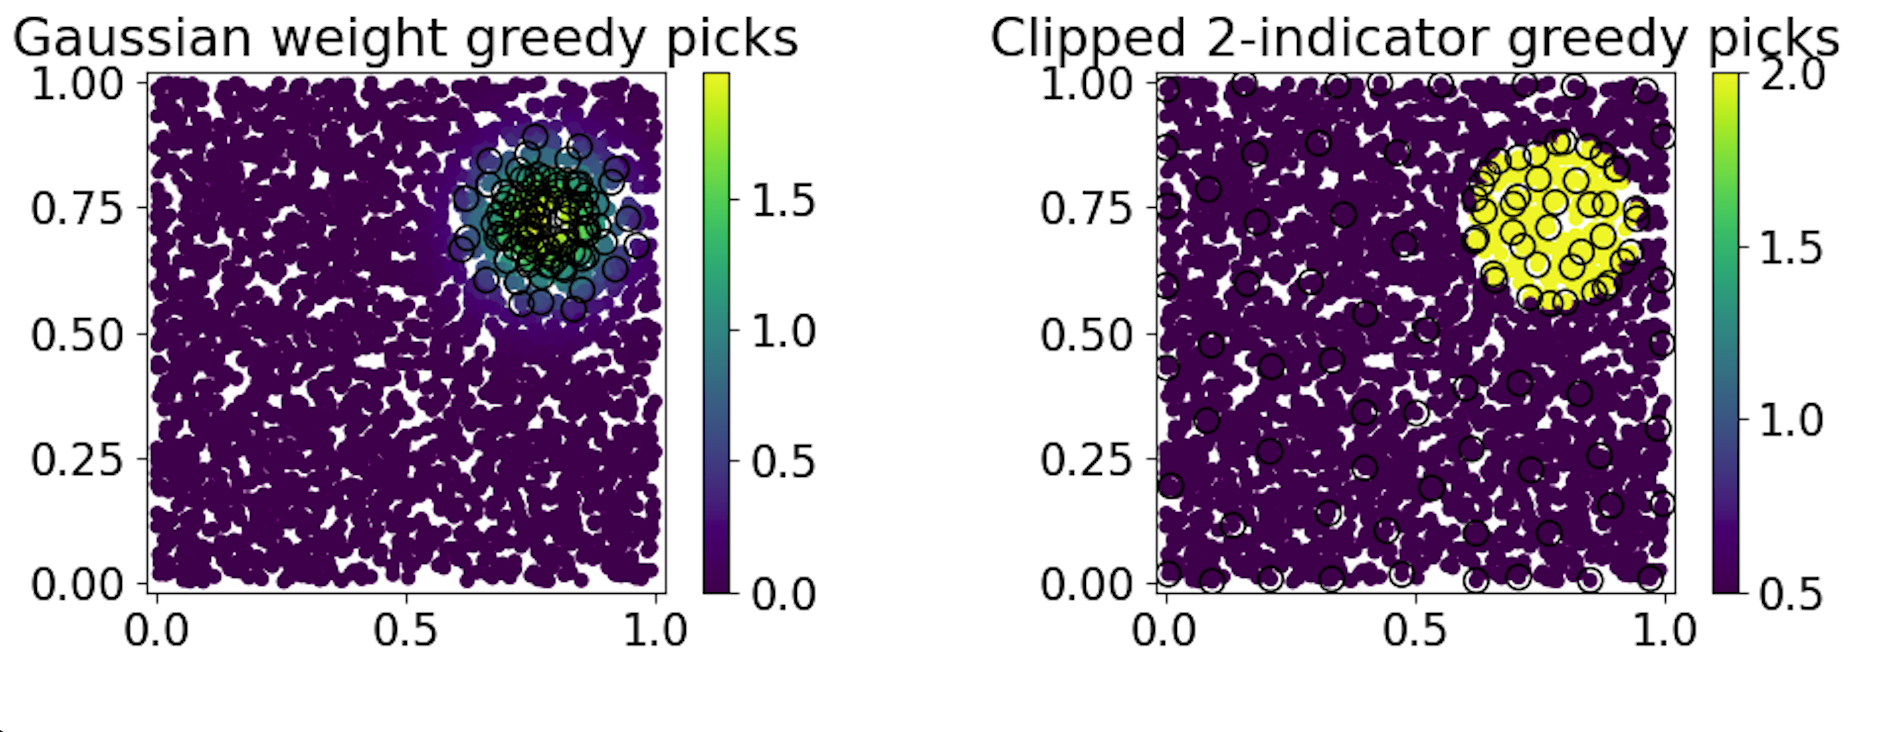
\includegraphics[width=0.9\linewidth]{point1.png}
\caption{
Gaussian weight centred at a point and the corresponding clipped two-region overestimate. Circles indicate the locations selected by the greedy weighted design.
}
\label{fig:point_geometry}
\end{figure}

Figure~\ref{fig:point_geometry} shows that both weighting schemes concentrate the selected points near the region of interest. Under the Gaussian weight, $93$ of the $100$ selected points lie inside the high-weight region.

The resulting greedy weighted objectives were
\begin{equation*}
\Gamma_{\mathrm{gauss}}^{\mathrm{greedy}}
=
65.89,
\qquad
\Gamma_{\mathrm{clip}}^{\mathrm{greedy}}
=
204.85.
\end{equation*}

The optimal split occurred at $m=22$, yielding
\begin{equation*}
\widehat B_{\mathrm{split}}
=
213.03,
\end{equation*}
compared with the crude bound
\begin{equation*}
\widehat B_{\mathrm{crude}}
=
385.29.
\end{equation*}

Thus the split bound reduces the crude bound by approximately $45\%$.

\begin{figure}[H]
\centering
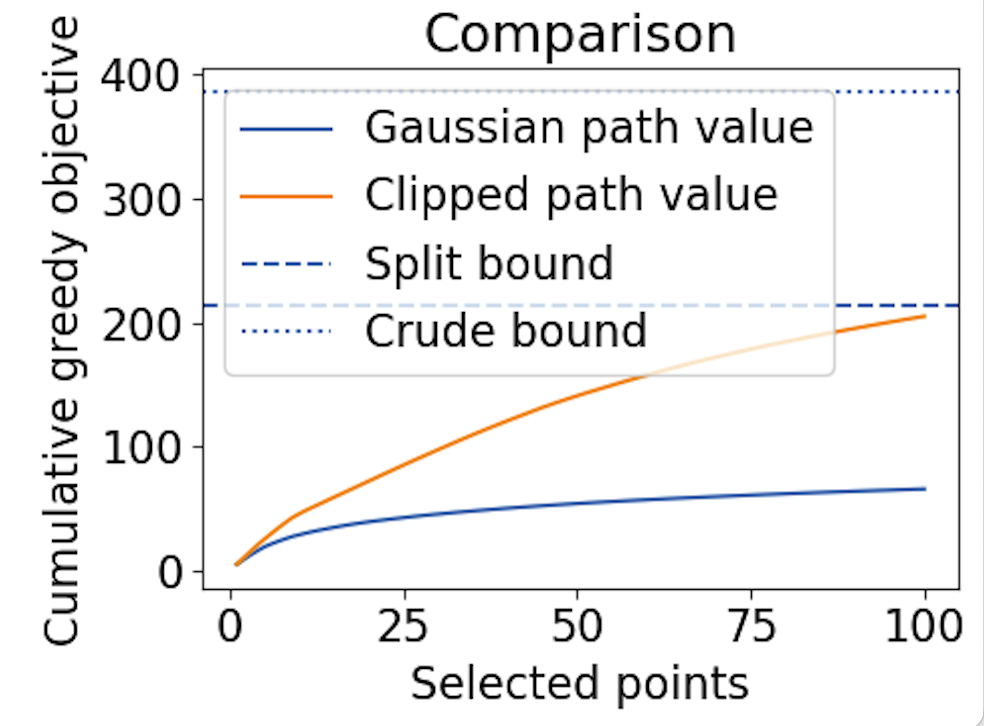
\includegraphics[width=0.5\linewidth]{point2.png}
\caption{
Cumulative greedy objective values together with the split and crude bounds.
}
\label{fig:point_bounds}
\end{figure}

Figure~\ref{fig:point_bounds} shows that the split bound tracks the clipped-weight objective much more closely than the crude max-weight bound. The improvement arises because the high-weight region occupies only a small fraction of the domain, allowing the regional decomposition to exploit this localisation.

\subsection{High-weight tube around a one-dimensional structure}

Our second experiment considers a weight concentrated around the line
\begin{equation*}
L=\{(x,y)\in[0,1]^2:y=0.5\}.
\end{equation*}

The Gaussian weight is defined by
\begin{equation*}
w_{\mathrm{gauss}}(x,y)
=
a
\exp\!\left(
-\frac{d_L(x,y)^2}{2s^2}
\right),
\end{equation*}
where
\begin{equation*}
d_L(x,y)=|y-0.5|.
\end{equation*}

The corresponding clipped overestimate is obtained using the same parameters as in the previous experiment. This produces a high-weight band containing $774$ candidate points and a background region containing $2226$ candidate points.

\begin{figure}[H]
\centering
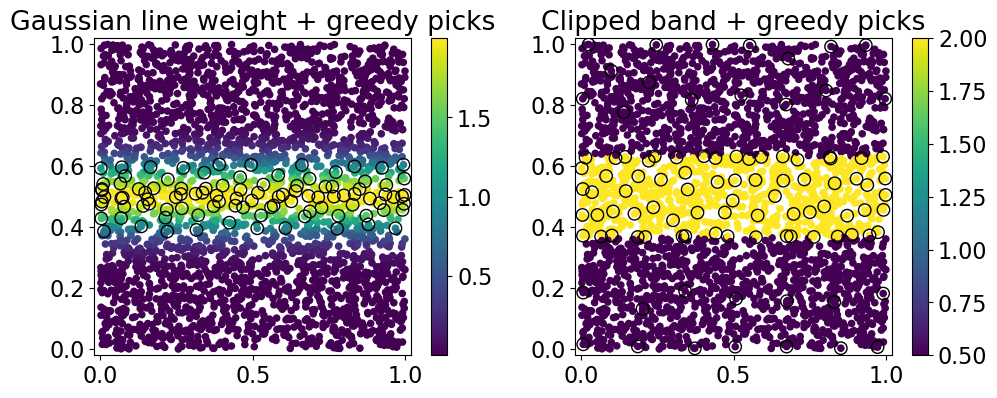
\includegraphics[width=0.9\linewidth]{line1.png}
\caption{
Gaussian line weight and clipped band approximation together with the greedy sampling locations.
}
\label{fig:line_geometry}
\end{figure}

As shown in Figure~\ref{fig:line_geometry}, the greedy weighted design strongly concentrates its samples inside the band. Under the Gaussian weight all $100$ selected points lie inside the high-weight region.

The greedy weighted objectives were
\begin{equation*}
\Gamma_{\mathrm{gauss}}^{\mathrm{greedy}}
=
165.60,
\qquad
\Gamma_{\mathrm{clip}}^{\mathrm{greedy}}
=
264.61.
\end{equation*}

The best split occurred at $m=42$, yielding
\begin{equation*}
\widehat B_{\mathrm{split}}
=
271.16,
\end{equation*}
while the crude bound remained
\begin{equation*}
\widehat B_{\mathrm{crude}}
=
385.29.
\end{equation*}

This corresponds to a reduction of approximately $30\%$.

\begin{figure}[H]
\centering
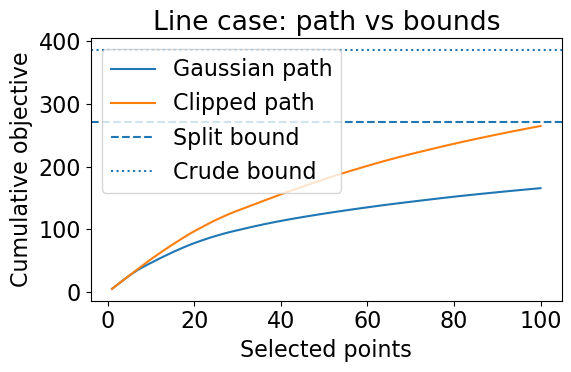
\includegraphics[width=0.5\linewidth]{line2.png}
\caption{
Cumulative greedy objective values together with the split and crude bounds.
}
\label{fig:line_bounds}
\end{figure}

\subsection{Discussion}

Both experiments exhibit a substantial gap between the split and crude
bounds. The effect is strongest in the first experiment, where the
high-weight region occupies a small localised subset of the domain and
the split bound improves the crude bound by approximately $45\%$.

In the second experiment the high-weight region occupies a much larger
fraction of the domain, leading to a smaller but still significant
improvement of approximately $30\%$.

These observations are consistent with the theoretical results of the
previous sections. When the regions carrying the largest weights occupy
only a small portion of the domain, analysing them separately can yield
considerably tighter information-gain estimates than treating the entire
domain as though it were weighted uniformly by the largest weight.



\section{Kernel-specific bounds}

The final step is to combine the split bound with existing kernel-specific
information gain estimates. We primarily follow the analysis of
Srinivas et al.~\cite{Srinivas2009}, who derive bounds on the maximum
information gain for several commonly used kernels using spectral decay
properties of the corresponding kernel operators. 

Unlike the original asymptotic bounds, we keep geometric constants explicit,
since in the split-bound setting the information gain terms are evaluated
on different regions of the domain. As a result, quantities such as the
effective dimension and volume-dependent constants may vary between
regions and contribute to the improvement obtained by the split bound in the finite-horizon setting.

\subsection{Linear kernel}

For the linear kernel
\begin{equation*}
k(x,x')
=
x^\top x',
\qquad
x\in\mathbb R^d,
\end{equation*}
the information gain admits a finite-rank bound. We again retain the geometric dependence explicitly, since in the split-bound setting the relevant radius may vary across regions.

\subsubsection{Standard finite-rank bound}

Starting from the log-determinant representation,
\begin{equation*}
\Gamma_T
=
\frac12
\max_{x_1,\dots,x_T}
\log\det
\left(
I+\sigma^{-2}X_T^\top X_T
\right),
\end{equation*}
where
\begin{equation*}
X_T
=
\begin{bmatrix}
x_1^\top \\
\vdots \\
x_T^\top
\end{bmatrix},
\end{equation*}
we use the identity
\begin{equation*}
\det(I+A^\top A)
=
\det(I+AA^\top)
\end{equation*}
to obtain
\begin{equation*}
\Gamma_T
=
\frac12
\max_{x_1,\dots,x_T}
\log\det
\left(
I+\sigma^{-2}X_TX_T^\top
\right).
\end{equation*}

Let the eigenvalues of $X_T^\top X_T$ be $\lambda_1,\dots,\lambda_d$.
Assuming $\|x_t\|\leq 1$, we have
$$
\operatorname{tr}(X_T^\top X_T)
=
\sum_{t=1}^T
\|x_t\|^2
\leq
T,
$$
and therefore
$$
\sum_{i=1}^d \lambda_i \leq T.
$$

Now,
\begin{equation*}
\log\det
\left(
I+\sigma^{-2}X_TX_T^\top
\right)
=
\sum_{i=1}^d
\log(1+\sigma^{-2}\lambda_i).
\end{equation*}
Since $\log(1+x)$ is concave, the sum is maximised by spreading the mass uniformly,
$
\lambda_i
=
\frac{T}{d},$
giving
\begin{equation*}
\Gamma_T
\leq
\frac{d}{2}
\log
\left(
1+\frac{T}{d\sigma^2}
\right).
\end{equation*}
This is the standard finite-rank information gain bound; see, for example, \cite{Srinivas2009}.

\subsubsection{Radius-dependent refinement}

The previous bound assumes
\begin{equation*}
\|x_t\|\leq 1.
\end{equation*}
To make the geometric dependence explicit, we instead abandon this normalisation and introduce the centred linear kernel
\begin{equation*}
k_c(x,x')
=
(x-c)^\top(x'-c).
\end{equation*}

\begin{proposition}[Radius-dependent linear kernel bound]
Suppose a region $A$ lies inside a ball of radius $R$ centred at $c$, so that
\begin{equation*}
\|x-c\|\leq R
\qquad
\text{for all } x\in A.
\end{equation*}
Then
\begin{equation*}
\Gamma_T(R,\sigma^2)
\leq
\frac{d}{2}
\log
\left(
1+\frac{TR^2}{d\sigma^2}
\right).
\end{equation*}
In the weighted setting, replacing $\sigma^2$ by the effective noise level $\sigma^2/w^2$
gives
\begin{equation*}
\Gamma_T(R,\sigma^2/w^2)
\leq
\frac{d}{2}
\log
\left(
1+\frac{TR^2w^2}{d\sigma^2}
\right).
\end{equation*}
\end{proposition}

\subsubsection{Crude versus split bound}

Applying Proposition~\ref{prop: splitbound} together with the radius-dependent estimate yields the following explicit two-region bound.

\begin{corollary}[Linear split bound for concentric regions]
Consider two concentric regions:
\begin{itemize}
    \item an inner ball $A$ of radius $R_1$ with weight $w_1$,
    \item an outer annulus $B$ extending to radius $R_2$ with weight $w_2$,
\end{itemize}
with $w_1>w_2.$ Then
\begin{equation*}
B_{\mathrm{split}} =
\max_{m=0,\dots,T}
\Bigg\{
\frac{d}{2}
\log
\left(
1+\frac{mR_1^2w_1^2}{d\sigma^2}
\right)
+
\frac{d}{2}
\log
\left(
1+\frac{(T-m)R_2^2w_2^2}{d\sigma^2}
\right)
\Bigg\},
\end{equation*}
whereas the corresponding crude bound is
\begin{equation*}
B_{\mathrm{crude}}
=
\frac{d}{2}
\log
\left(
1+\frac{TR_2^2w_1^2}{d\sigma^2}
\right).
\end{equation*}
\end{corollary}

\begin{remark}[Geometric separation]
The crude bound combines the largest weight and largest radius globally. By contrast, the split bound separates the geometric contributions of the different regions. Consequently, highly weighted regions contribute through the smaller radius $R_1$ rather than the global radius $R_2$.
\end{remark}

\subsubsection{Continuous relaxation and bound comparison}

Write
\begin{equation*}
a_0
=
\frac{R_1^2w_1^2}{d\sigma^2},
\qquad
b_0
=
\frac{R_2^2w_2^2}{d\sigma^2}.
\end{equation*}
Then the linear split bound is
\begin{equation*}
B_{\mathrm{split}}
=
\max_{m=0,\dots,T}
\frac{d}{2}
\left[
\log(1+a_0m)
+
\log(1+b_0(T-m))
\right].
\end{equation*}

\begin{lemma}[Continuous maximiser of the split allocation]
Treating $m$ as continuous, the split bound is maximised at
\begin{equation*}
m^\star=
\frac{T}{2}
+
\frac{1}{2b_0}
-
\frac{1}{2a_0}
=
\frac{T}{2}
+
\frac{d\sigma^2}{2R_2^2w_2^2}
-
\frac{d\sigma^2}{2R_1^2w_1^2}.
\end{equation*}
\end{lemma}

\begin{proof}
The derivative vanishes when
\begin{equation*}
\frac{a_0}{1+a_0m}
=
\frac{b_0}{1+b_0(T-m)}.
\end{equation*}
Solving for $m$ gives the stated expression.
\end{proof}
Thus the ``worst case'' integer allocation for the split bound is obtained by projecting $m^\star$ onto $[0,T]$ and rounding to the nearest integer. In particular, increasing $R_1^2w_1^2$ shifts the maximiser toward larger allocations in the high-weight region, while increasing $R_2^2w_2^2$ shifts it toward the outer region.

\begin{corollary}[Comparison between crude and split bounds]
The continuous relaxation satisfies
\begin{align*}
B_{\mathrm{split}}
&\leq
\frac{d}{2}
\log
\left(
\left(
1+\frac{a_0T}{2}+\frac{a_0}{2b_0}-\frac12
\right)
\left(
1+\frac{b_0T}{2}+\frac{b_0}{2a_0}-\frac12
\right)
\right),
\end{align*}
and therefore
\begin{align*}
B_{\mathrm{crude}}-B_{\mathrm{split}}
&\geq
\frac{d}{2}
\log
\Bigg(
\frac{
1+\dfrac{TR_2^2w_1^2}{d\sigma^2}
}{
\left(
\frac12
+
\dfrac{TR_1^2w_1^2}{2d\sigma^2}
+
\dfrac{R_1^2w_1^2}{2R_2^2w_2^2}
\right)
\left(
\frac12
+
\dfrac{TR_2^2w_2^2}{2d\sigma^2}
+
\dfrac{R_2^2w_2^2}{2R_1^2w_1^2}
\right)
}
\Bigg).
\end{align*}
\end{corollary}

\begin{proof}
Substituting $m^\star$ into the continuous relaxation gives
\begin{align*}
B_{\mathrm{split}}
&\leq
\frac{d}{2}
\log
\left(
\left(
1+a_0 m^\star
\right)
\left(
1+b_0(T-m^\star)
\right)
\right),
\end{align*}
which simplifies to the stated expression. Comparing with
\begin{equation*}
B_{\mathrm{crude}}
=
\frac{d}{2}
\log(1+a_0TR_2^2/R_1^2)
\end{equation*}
gives the result.
\end{proof}

The comparison becomes particularly transparent in the regime where the high-weight region is geometrically concentrated.
In particular, this shows that the crude bound is large because it combines the largest radius and largest weight. The split bound avoids this worst-case combination: the high weight $w_1$ is paired only with the smaller radius $R_1$, while the larger radius $R_2$ is paired with the smaller weight $w_2$. Thus the split bound can improve substantially when
\begin{equation*}
R_1^2
\ll
R_2^2
\qquad
\text{and}
\qquad
w_2^2
\ll
w_1^2,
\end{equation*}
that is, when the highly weighted region is geometrically small and the large outer region has much smaller weight.

\subsection{Squared exponential kernel}
We now instantiate Theorem~8 of Srinivas et al.~\cite{Srinivas2009} for the SE kernel, closely following the argument that appears there. However, unlike the original presentation, we retain the geometric and discretisation constants explicitly rather than absorbing them into asymptotic notation. This becomes important in the split-bound setting, where the information gain is evaluated on smaller regions of the domain. In particular, both the effective dimension and the volume-dependent discretisation constants may change from region to region, so the constants themselves can contribute meaningfully to improvements in the resulting bounds.

\subsubsection{Instantiation of Theorem~8}

For the SE kernel, the eigenvalue tail satisfies
\begin{equation*}
B_k(T_*)
=
\mathcal{O}
\left(
e^{-\beta}\beta^{d-1}
\right),
\qquad
\beta
=
\alpha T_*^{1/d},
\end{equation*}
as shown by Seeger et al.~\cite{Seeger2008}. As in Srinivas et al., we choose $J=d$, for which the discretisation term becomes constant.

Following the proof of Theorem~8, choose $T_*$ such that
\begin{equation*}
e^{-\beta}
=
(Tn_T)^{-1},
\end{equation*}
with
\begin{equation*}
n_T
=
C_4T^d\log T.
\end{equation*}
Equivalently,
\begin{equation*}
\beta
=
\log(Tn_T)
=
\log(C_4T^{d+1}\log T),
\end{equation*}
so that
\begin{equation*}
T_*
=
\left(
\frac{
\log(C_4T^{d+1}\log T)
}{\alpha}
\right)^d.
\end{equation*}

Substituting into Theorem~8 gives
\begin{equation*}
\Gamma_T
\leq
\max_{r=1,\dots,T}
\left(
T_*
\log\!\left(
\frac{rn_T}{\sigma^2}
\right)
+
\sigma^{-2}
(1-r/T)
\left(
C_5\beta^{d-1}
+
C_4\log T
\right)
\right).
\end{equation*}
As in Srinivas et al., the first term dominates, so the maximum is attained at $r=T$. Hence
\begin{equation*}
\Gamma_T
\leq
T_*
\log\!\left(
\frac{Tn_T}{\sigma^2}
\right).
\end{equation*}

\subsubsection{Keeping constants $C_4$ and the dimension $d$ explicit}

\begin{proposition}[SE information gain bound with explicit constants]
For the Squared Exponential kernel,
\begin{equation}
\Gamma_T
=
\mathcal{O}
\left(
\left(
(d+1)\log T+\log C_4
\right)^d
\left(
(d+1)\log T+\log(C_4/\sigma^2)
\right)
\right).
\label{eq: SEdecayrate}
\end{equation}
\end{proposition}

\begin{proof}
Substituting the expression for $T_*$ gives
\begin{equation*}
\Gamma_T
\leq
\left(
\frac{
\log(C_4T^{d+1}\log T)
}{\alpha}
\right)^d
\log\!\left(
\frac{C_4T^{d+1}\log T}{\sigma^2}
\right).
\end{equation*}
Suppressing the lower-order $\log\log T$ term yields
\begin{equation*}
\Gamma_T
=
\mathcal{O}
\left(
\left(
(d+1)\log T+\log C_4
\right)^d
\left(
(d+1)\log T+\log(C_4/\sigma^2)
\right)
\right),
\end{equation*}
proving \eqref{eq: SEdecayrate}.
\end{proof}

\begin{remark}[Effect of volume and intrinsic dimension]

Expanding the first factor,
\begin{equation*}
\left(
(d+1)\log T+\log C_4
\right)^d
=
\sum_{k=0}^d
\binom{d}{k}
\left(
(d+1)\log T
\right)^{d-k}
(\log C_4)^k,
\end{equation*}
so that
\begin{equation*}
\Gamma_T
=
\mathcal{O}
\left(
\sum_{k=0}^d
\left(
(d+1)\log T
\right)^{d-k}
(\log C_4)^k
\left(
(d+1)\log T+\log(C_4/\sigma^2)
\right)
\right).
\end{equation*}

Asymptotically, if $C_4$ and $d$ are fixed, the leading term remains the $\mathcal{O}\left((d+1)^{d+1}(\log T)^{d+1}\right)$
rate. In particular, the volume dependence (entering through the geometric discretisation constant $C_4$) disappears entirely from the leading asymptotic exponent, surviving only as a lower-order logarithmic correction. This means that even large geometric changes affect the information gain much more mildly than changes in the effective dimension, which appears in the exponent of the logarithmic rate. 

This mild geometric dependence is closely tied to the exceptionally fast spectral decay of the SE kernel. Since the eigenvalues decay exponentially, geometric quantities such as the volume constant $C_4$ survive only inside logarithms, whereas the intrinsic dimension $d$ still appears in the exponent of the overall rate. By contrast, for rougher kernels such as Mat\'ern kernels, where the eigenvalue decay is only polynomial, one expects the geometry and intrinsic dimension of the regions to have a substantially stronger effect on the resulting information gain bounds.

However, for finite $T$, the constant-dependent and dimension-dependent terms can still be significant. This is especially relevant for the split bound, where different regions may have different effective geometric constants and possibly different effective dimensions.

For example, suppose that in one regional bound the effective constant is large enough that
\begin{equation*}
\log C_4 \approx (\log T)^m,
\qquad
m\geq 1.
\end{equation*}
Substituting this into a typical term of the expanded bound gives
\begin{align*}
&\left(
(d+1)\log T
\right)^{d-k}
(\log C_4)^k
\left(
(d+1)\log T+\log(C_4/\sigma^2)
\right) \\
& \qquad \qquad \approx
(d+1)^{d-k}
(\log T)^{d-k+mk}
\left(
(d+1)\log T+(\log T)^m-\log\sigma^2
\right).
\end{align*}
Thus the exponent of $\log T$ in the first factor is
\begin{equation*}
d-k+mk
=
d+(m-1)k,
\end{equation*}
which increases with $k$ whenever $m>1$. Hence constant-dependent terms can be of order
\begin{equation*}
(d+1)^{d-k}
(\log T)^{d+(m-1)k+m},
\end{equation*}
which may dominate the nominal leading term
\begin{equation*}
(d+1)^{d+1}(\log T)^{d+1}
\end{equation*}
for finite $T$, illustrating why these constants should not be hidden in the present setting. \end{remark}

\subsubsection{Regional refinements of the information gain bound}

For the SE kernel, the dimensional dependence is itself geometric. If the kernel is restricted to a lower-dimensional manifold $M\subseteq\mathbb R^D$, the restricted kernel agrees with the corresponding lower-dimensional SE kernel on $M$, since the collapsed coordinates do not contribute to the Euclidean distance. Consequently, one may expect the associated eigenvalue decay, and hence the information gain bound, to depend on the intrinsic dimension of the subset rather than the ambient dimension. This suggests that restricting the split bound to highly weighted lower-dimensional regions could yield substantially sharper rates.

Furthermore, in the proof of Theorem~8, the discretisation size is chosen as
\begin{equation*}
n_T
=
C_4T^\tau\log T,
\qquad
C_4
=
2\mathcal{V}(D)(2\tau+1),
\end{equation*}
so $C_4$ depends directly on the geometry of the domain through its volume $\mathcal{V}(D)$. Consequently, when applying the split bound to smaller regions or lower-dimensional subsets, one may obtain improvements not only through the effective dimension but also through smaller volume-dependent discretisation constants.  We will illustrate this by plugging our constant-dependent rate \eqref{eq: SEdecayrate} into Proposition~\ref{prop: splitbound}.

\begin{corollary}[SE split bound with regional geometry]
Consider the two-region weighting
\begin{equation*}
w(x)
=
w_1\mathbf 1_A(x)
+
w_2\mathbf 1_B(x),
\qquad
w_1>w_2.
\end{equation*}
Suppose the restrictions of the SE kernel to $A$ and $B$ have effective dimensions $d_A,d_B$ and discretisation constants
\begin{equation*}
C_{4,A}
=
2\mathcal V(A)(2\tau+1),
\qquad
C_{4,B}
=
2\mathcal V(B)(2\tau+1).
\end{equation*}
Then Proposition~\ref{prop: splitbound} together with the SE kernel estimate \eqref{eq: SEdecayrate} yields
\begin{align*}
\Gamma_T^w
\leq
\max_{m=0,\dots,T}
\Bigg\{
&
\mathcal O
\Big(
\big(
(d_A+1)\log m+\log C_{4,A}
\big)^{d_A}
\\
&\qquad\qquad\qquad\qquad \times
\big(
(d_A+1)\log m
+
\log(C_{4,A}w_1^2/\sigma^2)
\big)
\Big)
\\
+
&
\mathcal O
\Big(
\big(
(d_B+1)\log(T-m)+\log C_{4,B}
\big)^{d_B}
\\
&\qquad\qquad\qquad\qquad \times
\big(
(d_B+1)\log(T-m)
+
\log(C_{4,B}w_2^2/\sigma^2)
\big)
\Big)
\Bigg\}.
\end{align*}
By comparison, the crude bound satisfies
\begin{align*}
\Gamma_T^w
\leq
\mathcal O
\Big(
\big(
(D+1)\log T+\log C_{4,\mathcal X}
\big)^D
\\
\times
\big(
(D+1)\log T
+
\log(C_{4,\mathcal X}w_1^2/\sigma^2)
\big)
\Big),
\end{align*}
where $D$ is the ambient dimension and
\begin{equation*}
C_{4,\mathcal X}
=
2\mathcal V(\mathcal X)(2\tau+1).
\end{equation*}
\end{corollary}
\paragraph{Benefit from smaller regional volume.}

Suppose the highly weighted region $A$ occupies only a small subset of the full domain. Then
\begin{equation*}
\mathcal V(A)\ll \mathcal V(\mathcal X),
\end{equation*}
so the corresponding discretisation constant satisfies
\begin{equation*}
C_{4,A}\ll C_{4,\mathcal X}.
\end{equation*}
Since the volume dependence enters only logarithmically, the improvement is lower-order asymptotically. However, for finite $T$, sufficiently large differences in regional volume can still produce substantial reductions in the bound.

\paragraph{Effect of lower effective dimension.}
If the highly weighted region lies on a lower-dimensional subset, so that
\begin{equation*}
d_A<D,
\end{equation*}
then the improvement is substantially stronger, since the effective dimension appears in the exponent of the logarithmic rate itself:
\begin{equation*}
(\log T)^{D+1}
\quad\longrightarrow\quad
(\log T)^{d_A+1}.
\end{equation*}

Thus the split bound can exploit both smaller regional volume and lower intrinsic dimension, with the dimensional effect dominating asymptotically.

\subsection{Mat\'ern kernel}

We now instantiate Theorem~8 of Srinivas et al.~\cite{Srinivas2009} for the Mat\'ern kernel. As in \cite{Srinivas2009}, using the eigenvalue decay estimates of Seeger et al.~\cite{Seeger2008}, the eigenvalues satisfy
\begin{equation*}
\lambda_s
\leq
c\,s^{-(2\nu+d)/d},
\end{equation*}
and hence the eigenvalue tail obeys
\begin{equation*}
B_k(T_*)
=
\mathcal{O}
\left(
T_*^{-2\nu/d}
\right).
\end{equation*}

Following Srinivas et al., choose
\begin{equation*}
T_*
=
(Tn_T)^{d/(2\nu+d)}
\left(
\log(Tn_T)
\right)^{-d/(2\nu+d)}.
\end{equation*}
Substituting $n_T=C_4T^\tau\log T$ gives
\begin{equation*}
T_*
=
\left(
C_4T^{\tau+1}\log T
\right)^{d/(2\nu+d)}
\left(
\log(C_4T^{\tau+1}\log T)
\right)^{-d/(2\nu+d)}.
\end{equation*}

The dominant term in Theorem~8 is therefore
\begin{equation*}
T_*
\log\left(
\frac{Tn_T}{\sigma^2}
\right),
\end{equation*}
which becomes
\begin{equation}  \label{eq: dominantterm}
\mathcal{O}
\left(
\left(
C_4T^{\tau+1}\log T
\right)^{d/(2\nu+d)}
\left(
\log(C_4T^{\tau+1}\log T)
\right)^{-d/(2\nu+d)}
\log\left(
\frac{C_4T^{\tau+1}\log T}{\sigma^2}
\right)
\right).
\end{equation}

The remaining discretisation term in Theorem~8 is
\begin{equation*}
\mathcal{O}
\left(
T^{1-\tau/d}
\right).
\end{equation*}
To balance this with the dominant term \eqref{eq: dominantterm}, we choose $\tau$ so that the polynomial powers of $T$ agree:
\begin{equation*}
\frac{(\tau+1)d}{2\nu+d}
=
1-\frac{\tau}{d}.
\end{equation*}
Solving gives
\begin{equation}
\tau
=
\frac{2\nu d}{2\nu+d(d+1)}
\label{eq: materntao}
\end{equation}
 and with this choice,
\begin{equation*}
\frac{(\tau+1)d}{2\nu+d}
=
\frac{d(d+1)}{2\nu+d(d+1)}.
\end{equation*}

\subsubsection{Constant-dependent rate}
\begin{proposition}[Mat\'ern information gain bound with explicit constants] \label{prop: maternexplicit}
Let
\begin{equation*}
\eta
=
\frac{\nu}{2\nu+d(d+1)}.
\end{equation*}
Then, suppressing lower-order logarithmic factors while retaining the explicit dependence on $C_4$ and $\sigma^2$,
\begin{equation*}
\Gamma_T
=
\mathcal{O}
\left(
C_4^{d/(2\nu+d)}
T^{1-2\eta}
\log\!\left(
\frac{C_4T^{\tau+1}}{\sigma^2}
\right)
\right).
\end{equation*}
\end{proposition}

\begin{proof}
Substituting \eqref{eq: materntao} into \eqref{eq: dominantterm} yields
\begin{equation*}
\Gamma_T
=
\mathcal{O}
\left(
C_4^{d/(2\nu+d)}
T^{\frac{d(d+1)}{2\nu+d(d+1)}}
(\log T)^{d/(2\nu+d)}
\left(
\log(C_4T^{\tau+1}\log T)
\right)^{-d/(2\nu+d)}
\log\!\left(
\frac{C_4T^{\tau+1}\log T}{\sigma^2}
\right)
\right).
\end{equation*}

Since
\begin{equation*}
\frac{d(d+1)}{2\nu+d(d+1)}
=
1-2\eta,
\end{equation*}
and
\begin{equation*}
(\log T)^{d/(2\nu+d)}
\left(
\log(C_4T^{\tau+1}\log T)
\right)^{-d/(2\nu+d)}
=
\Theta(1),
\end{equation*}
the claimed bound follows.
\end{proof}

\begin{remark}[Effect of volume and intrinsic dimension]
Unlike the SE kernel, the Mat\'ern kernel exhibits only polynomial spectral decay. Consequently, the geometric discretisation constant $C_4$ enters as the polynomial factor
\begin{equation*}
C_4^{d/(2\nu+d)},
\end{equation*}
rather than only through logarithmic corrections. Similarly, the effective dimension appears directly in the polynomial exponent
\begin{equation*}
1-\frac{2\nu}{2\nu+d(d+1)}.
\end{equation*}
Thus reductions in volume and intrinsic dimension can affect the leading-order behaviour of the information gain bound.
\end{remark}

\subsubsection{Regional decomposition of the information gain}

\begin{corollary}[Mat\'ern split bound with regional geometry]
Consider the two-region weighting
\begin{equation*}
w(x)
=
w_1\mathbf 1_A(x)
+
w_2\mathbf 1_B(x),
\qquad
w_1>w_2.
\end{equation*}

Suppose the restrictions of the Mat\'ern kernel to $A$ and $B$
have effective dimensions $d_A,d_B$ and discretisation constants
$C_{4,A},C_{4,B}$.

Then applying Proposition~\ref{prop: maternexplicit} separately on each region with Proposition~\ref{prop: splitbound}
gives
\begin{equation*}
\Gamma_T^w
\le
\max_{m=0,\ldots,T}
\Big\{
C_{4,A}^{d_A/(2\nu+d_A)}
m^{1-2\eta_A}
\log\!\Big(
\frac{C_{4,A}m^{\tau_A+1}}{\sigma^2/w_1^2}
\Big)
\end{equation*}
\begin{equation*}
+
C_{4,B}^{d_B/(2\nu+d_B)}
(T-m)^{1-2\eta_B}
\log\!\Big(
\frac{C_{4,B}(T-m)^{\tau_B+1}}
{\sigma^2/w_2^2}
\Big)
\Big\},
\end{equation*}
where
\begin{equation*}
\eta_i
=
\frac{\nu}
{2\nu+d_i(d_i+1)}
\end{equation*}
and 
$$\tau_i=\frac{2 \nu d_i}{2 \nu+d_i\left(d_i+1\right)}.$$
\end{corollary}


\paragraph{Effect of regional geometry.}

Since
\begin{equation*}
\Gamma_T
\propto
C_4^{d/(2\nu+d)},
\end{equation*}
a reduction in regional volume produces a direct polynomial reduction in the information gain bound. Unlike the SE case, this effect persists in the leading-order term.
Furthermore, if
\begin{equation*}
d_A<D,
\end{equation*}
then
\begin{equation*}
T^{1-\frac{2\nu}{2\nu+D(D+1)}}
\quad\longrightarrow\quad
T^{1-\frac{2\nu}{2\nu+d_A(d_A+1)}}.
\end{equation*}
Thus a lower-dimensional highly weighted region can improve the asymptotic polynomial growth rate itself, rather than merely reducing logarithmic factors as in the SE case.


\clearpage 

\section*{References}

\addcontentsline{toc}{section}{References}

\clearpage
\appendix

\appendixpage
\addappheadtotoc

\section{Heuristic approximation argument for the continuum limit} \label{appendix:continuum}


Let $w:\mathcal{X}\to \mathbb{R}_+$ be continuous and take a partition
\begin{equation*}
\mathcal{X}
=
\bigcup_{i=1}^{m_n}
A_i^{(n)},
\end{equation*}
where the mesh size tends to zero as $n\to\infty$.

Define the piecewise constant approximation
\begin{equation*}
w_n(x)
=
\sum_{i=1}^{m_n}
c_i^{(n)}
\mathbf{1}_{A_i^{(n)}}(x),
\end{equation*}
where either
\begin{equation*}
c_i^{(n)}
=
w(x_i^{(n)})
\end{equation*}
for some representative point
\begin{equation*}
x_i^{(n)}\in A_i^{(n)},
\end{equation*}
or alternatively
\begin{equation*}
c_i^{(n)}
=
\frac{1}{\mu(A_i^{(n)})}
\int_{A_i^{(n)}} w(x)\,d\mu(x).
\end{equation*}

The corresponding regional transductive objective is
\begin{equation*}
F_{w_n}(S)
=
\sum_{i=1}^{m_n}
c_i^{(n)}
I(f_{A_i^{(n)}};y_S).
\end{equation*}

One would like to understand whether these objectives converge, in a suitable sense, to a continuum limit as the partition is refined.

\paragraph{Local information density viewpoint}

Define
\begin{equation*}
\phi(A_i,S)
:=
\frac{1}{\mu(A_i)}
I(f_{A_i};y_S).
\end{equation*}
Then
\begin{equation*}
F_{w_n}(S)
=
\sum_i
c_i^{(n)}
\mu(A_i^{(n)})
\phi(A_i^{(n)},S).
\end{equation*}

Suppose
\begin{equation*}
\phi(A_i^{(n)},S)
\to
\psi(x_i,S)
\qquad
\text{as }
\mu(A_i^{(n)})\to 0
\end{equation*}
for some pointwise limit $\psi(x,S)$. Then
\begin{equation*}
F_{w_n}(S)
\approx
\sum_i
c_i^{(n)}
\mu(A_i^{(n)})
\psi(x_i,S),
\end{equation*}
which formally converges to the Riemann integral
\begin{equation*}
\int
w(x)\psi(x,S)\,d\mu(x).
\end{equation*}

\paragraph{Alternative averaged-field viewpoint}

Define
\begin{equation*}
\bar f_A
:=
\frac{1}{\mu(A)}
\int_A
f(x)\,d\mu(x).
\end{equation*}
If
\begin{equation*}
\bar f_{A_i^{(n)}}
\to
f(x_i)
\qquad
\text{as }
\mu(A_i^{(n)})\to 0,
\end{equation*}
then one might hope that
\begin{equation*}
I(\bar f_{A_i^{(n)}};y_S)
\to
I(f(x_i);y_S)
\qquad
\text{as }
n\to\infty.
\end{equation*}

Consequently,
\begin{equation*}
F_{w_n}(S)
=
\sum_i
c_i^{(n)}
\mu(A_i^{(n)})
I(\bar f_{A_i^{(n)}};y_S)
\approx
\sum_i
c_i^{(n)}
\mu(A_i^{(n)})
I(f(x_i);y_S),
\end{equation*}
which again formally converges to
\begin{equation*}
\int
w(x)\,
I(f(x);y_S)\,
d\mu(x).
\end{equation*}

At present, both of these approaches remain heuristic. The main difficulty is understanding the limiting behaviour of the transductive information terms as the regions shrink. In particular, it is not immediately clear under what regularity assumptions the mutual information associated with an entire region converges to a local pointwise quantity.

\end{document}